\documentclass[../report.tex]{subfiles}
\begin{document}	
	
\chapter{Introduction} 
	\section{Light for communication using optical fibers}
Communication and collective thinking are the key to the development of human civilization. This development is driven by data - “The new oil of this digital era”. With the advent of \gls{iot}, it has been estimated that by 2020 there will be 26 billion connected devices \cite{gartner_iot}, and all devices that can be connected will be connected. Today, only about 40\% \cite{internet_users} of the world’s population use the internet and the amount of data produced per minute in the internet through different channels is already growing exponentially. 

\begin{figure}[h]
	\centering
	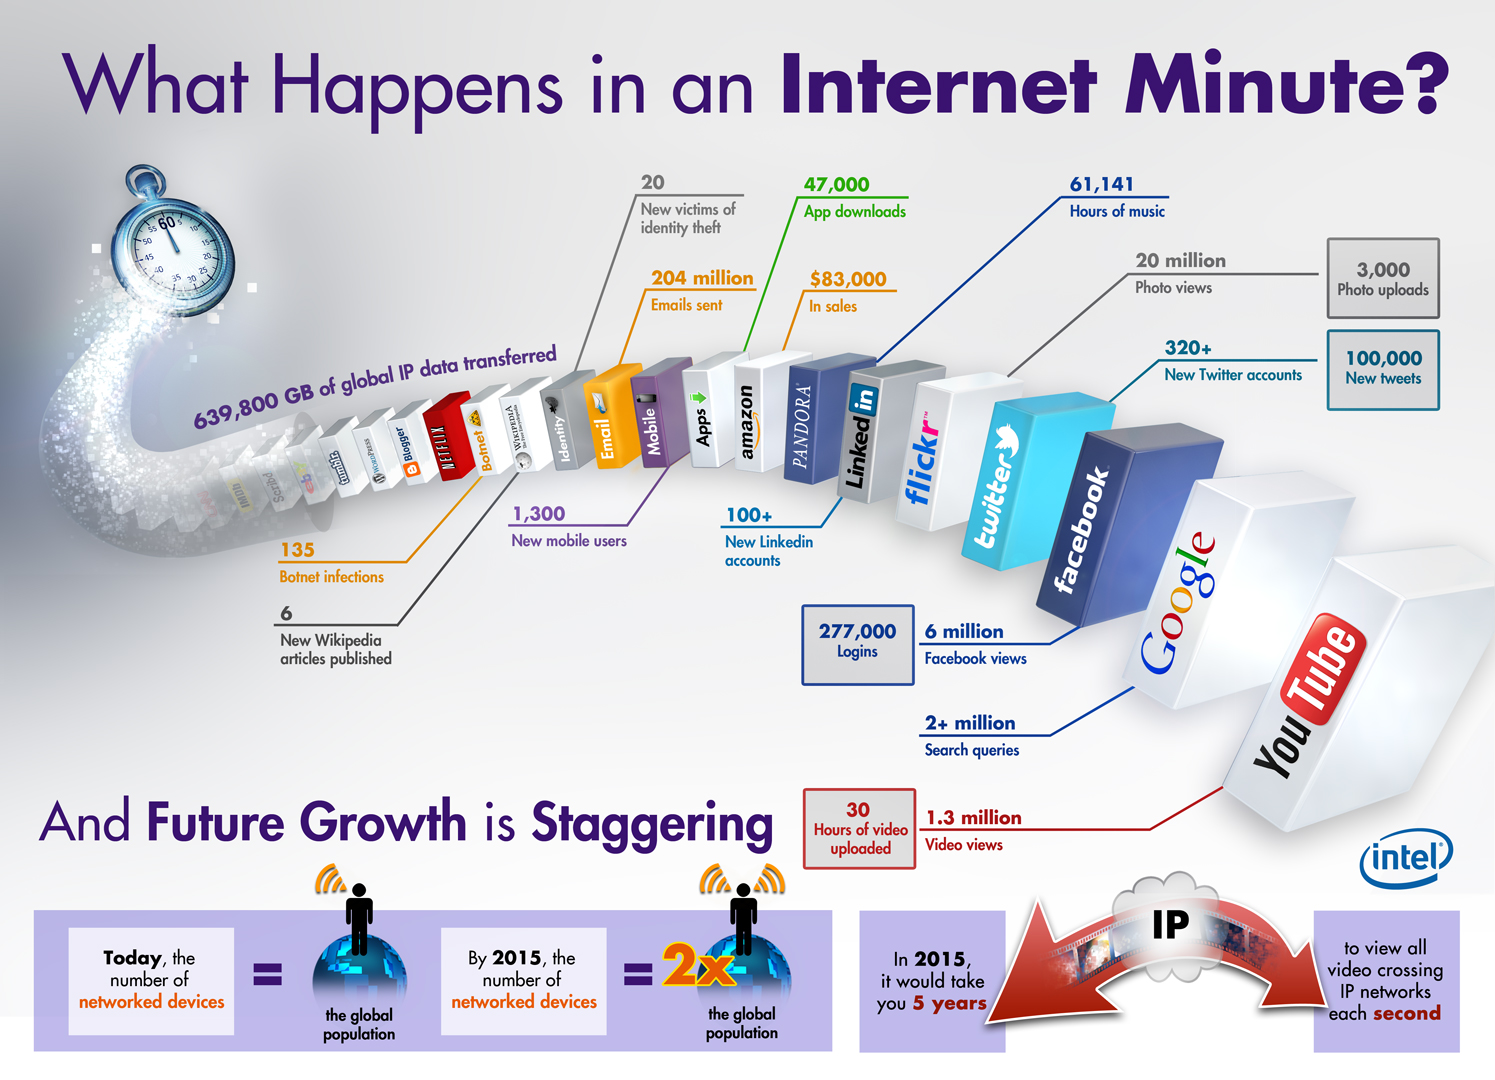
\includegraphics[width=0.75\textwidth]{1-Internet-minute}
	\caption{What happens on internet per minute \cite{internet_minute}}
	\label{fig:1_internet_minute}
\end{figure}
\noindent Eventually, as more and more people use the different \gls{ict} services, this data growth will be higher than ever. \par

Also, with the advent of smart-phones, there has been a huge surge in data traffic all over the world. It has been estimated in Ericsson's mobility report \cite{ericsson_mobility_report} that 70\% of world's population will use smart-phones by 2020 and 90\% of the world's population over 6 years old will have a mobile phone by 2020. 
\begin{figure}[!tbp]
	\centering
	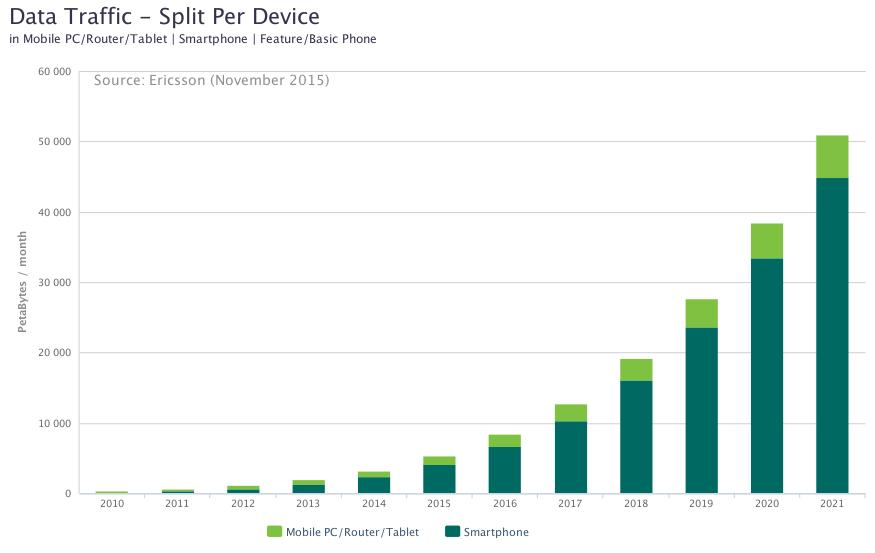
\includegraphics[width=1\textwidth]{1-data-traffic-forecast}
	\caption{Data traffic growth forecast by 2020, as per Ericsson, generated using \cite{ericsson_traffic_exploration} \cite{internet_minute}}
	\label{fig:1_data_traffic_forecast}
\end{figure}

Currently, the telecommunications industry is moving towards \gls{ims} core networks which is a transition towards full IP based networks. So how is this traffic managed? The answer is the optical fiber, which serves as the backbone of all the communication systems. Optical fiber is chosen over previously used copper cables for the following reasons:
\begin{itemize}
	\item[$\square$] Fiber provides more bandwidth than copper and has standardized performance up to 100 Gbps and beyond, at very low power.
	\item[$\square$] Fiber is also less susceptible to temperature fluctuations than copper and can be submerged in water for intercontinental long distance communication. It’s immune to \gls{em} interference and radio-frequency \gls{rf} interference, crosstalk, impedance problems etc. 
	\item[$\square$] It doesn’t radiate signals and is extremely difficult to tap, which provides better security than copper cables.
	\item[$\square$] Fiber optic transmission results in less attenuation than copper cables.
\end{itemize}

	\section{Silicon photonics for optical communication}
The performance of optical fiber network is remarkable and it is this backbone which gives us an unfathomable user experience. The current internet architecture has already pushed the optical fiber to the network edges and the trend is to push it as closer to the processor as possible. This has already opened up a new trend of “siliconizing photonics” \cite{silicon_photonics} based on the decades of research from microelectronics industry. The electronics industry has pushed the boundaries of the processing speed of \gls{ic} according to Moore’s Law, after the discovery of semiconductors. Until recently, exponential increases in the speed, efficiency, and processing power of conventional electronic devices were achieved largely through the downscaling and clustering of components on a chip. However, this trend toward miniaturization has yielded unwanted effects in the form of significant increases in noise, power consumption, signal propagation delay and aggravates already to serious thermal management problems. Alternatively, the wires can be made thicker, but then the packing density will be inefficient. As a result, traditional microelectronics will soon fall short of meeting market needs, inhibited by the thermal and bandwidth bottlenecks inherent in copper wiring. Intel processor speed and bus speed comparison \cite{intel_proc_compare} shows that although we have achieved good processing speed, the interconnects always find difficulty in catching up with the processing speed. Think of a data center processing \todo{have to make sure}tera-bytes of data per minute, where interconnects between processors can add up to a significant bottleneck. These bottlenecks can be overcome by substituting copper with optical interconnects using the current technology, which can also operate at low power and better efficiency. In addition optical interconnects can also reduce power consumption caused by heat dissipation, switching and transmission of electrical signals.\par

Although silicon is the optimal material for electronics, only recently silicon is being considered as a practical option for \gls{oeic} solutions. Silicon has many properties conducive to fiber optics. The band gap of silicon ($\sim$\SI{1.1}{\electronvolt}) is such that the material is transparent to wavelengths commonly used for optical transport ($\sim$\SI{1.3}{\micro\metre}-\SI{1.6}{\micro\metre}). One can use standard \gls{cmos} processing techniques to sculpt optical waveguides onto the silicon surface. Similar to an optical fiber, these waveguides can be used to confine and direct light as it passes through the silicon \cite{reed_silicon_2004} using total internal reflection. Due to the wavelengths typically used for optical transport and silicon’s high index of refraction, the feature sizes needed for processing these silicon waveguides are on the order of \SI{0.5}{\micro\metre}-\SI{1}{\micro\metre}. The fabrication and lithography requirements needed to process waveguides with these sizes exist today. Finally, if all this remains \gls{cmos}-compatible, it could be possible to process monolithic optical devices, which could bring new levels of performance, functionality, power and size reduction, all at a lower cost. \par

Today silicon photonics technology is a new approach to make optical devices out of silicon and use light (photons) to move huge amounts of data at very high speeds with extremely low power over a thin optical fiber rather than using electrical signals over a copper wire. Since, already enough capital investments has been done on perfecting the current fabrication technology and infrastructure, engineers are working on creating monolithic design of integrated circuits which will use light in place of electric signals \cite{optical_linking}. \todo{Previously, you had marked it when i wrote organization here}Research institutes in collaboration with industry partners, are trying to bridge this gap by creating highly integrated photonic and electronic components that combine the functionality of conventional \gls{cmos} circuits with the significantly enhanced system performance of photonic solutions. Various kinds of silicon photonic devices such as, switches \cite{wu_mems-enabled_2015,nikolova_scaling_2015,lu_low-power_2014}, modulators \cite{dong_silicon_2015,chen_generation_2013}, photodetectors \cite{urino_demonstration_2012,chang_high-power_2015}, delay lines \cite{garcia_design_2015,mattarei_variable_2014}, sensors \cite{janz_silicon_2007,lim_laser_2010,ryckeboer_glucose_2014} etc. have been reported till date. It is also promising in developing on-chip integration for telecommunications applications and servers in data centers \cite{jalali_silicon_2006}. The silicon photonics market is estimated to grow to 700 million USD by 2024 \cite{silicon_photonics_growth_2015} with a \gls{cagr} of 38\%. 

	\section{Motivation} 
All photonic devices based on silicon waveguides are sensitive to polarization due to large structural birefringence, which induces substantial \gls{pdl}, \gls{pmd}, and \gls{pdw}, limiting their usability. Also, in a complex \gls{oeic} system, polarization is a major issue because power can be exchanged between the polarization states in the presence of junctions, tapers, slanted sidewalls, bends, or other discontinuities. Therefore, sometimes, it is necessary to have a fixed degree of polarization state, and it may also be necessary to rotate an incoming polarization state.\par
To overcome these challenges, \gls{pr}s are engineered on silicon for \gls{oeic} and various designs have already been demonstrated \cite{xie_efficient_2015,velasco_ultracompact_2012,leung_numerical_2011,wang_design_2014,dai_novel_2011,wirth_efficient_2012,chen_compact_2011}. The main working principle of these proposed solutions is introducing asymmetry in the waveguide structure which changes the effective \gls{ri}. Also, in some cases the designs \cite{sarmiento-merenguel_demonstration_2015}, if used in commercial applications for miniature interconnects, would incur inefficient packing density since too much space is required to achieve high and robust tuning. Apart from that there might also be thermo-optic induction problem which might change phase of the wave in other waveguides in high compact density environment as silicon is highly susceptible to thermal changes \cite{ibrahim_athermal_2012}. Also, a \gls{tpr} has been reported which works on the principle of Berry’s phase, a quantum-mechanical phenomenon of purely topological origin \cite{xu_electrically_2014}. For \gls{pr}, the design uses out-of-plane ring cavity which inherits the narrow band spectral features of ring resonator limiting the bandwidth. Phase tuning is achieved through thermo-optic effect which has its limitations. The general goal of the thesis work is to realize an efficient \gls{tpr} using \gls{mems} in \todo{cross-check}C and L bands, at low power with high precision and accuracy.    
	\section{Objectives}
\textbf{Main objective}: To design and fabricate low power \gls{tpr} based on \gls{mems} tuning. \\

\noindent \textbf{Sub objectives}: The areas which will be addressed are:
\begin{itemize}
	\item[$\square$] Feasibility of the idea and the strategy to design the \gls{pr}. 
	\item[$\square$] Design and simulation of the device.
	\item[$\square$] Fabrication and characterization of the MEMS tunable \gls{pr}.
\end{itemize}
	
	\section{Outline of this thesis}
The outline of the thesis is as follows: Background, motivation and the research questions being addressed, is discussed in Chapter 1. In Chapter 2, the current state of art for the available solution is discussed along with the background literature required. Here, also the working principle of the current available design are explained along with the areas which can be improved. Chapter 3 discusses about the design of the final system and the results obtained about the simulation setup. In Chapter 4, documentation about the fabricated design is provided along with currently available standard fabrication technologies. Results and characterization are an important part of the work, which is discussed in Chapter 5. Finally, Chapter 6 and 7 discusses about the conclusion and future work possibilities respectively along with the known limitations of the system if any.  
	
\end{document}
